\documentclass[a4paper,10pt]{jsarticle}
\renewcommand{\figurename}{Fig.}
\renewcommand{\tablename}{Table }
\usepackage[left=2cm,right=2cm,top=3cm,bottom=3cm]{geometry}
\usepackage{multicol}
\usepackage{blindtext}
\usepackage{amsmath,amsfonts}
\usepackage{amssymb}
\usepackage{bm}
\usepackage{siunitx}
\usepackage[dvipdfmx]{graphicx}
\usepackage{booktabs}
\usepackage{multirow}
\usepackage{here}
\usepackage{wrapfig}
\usepackage{siunitx}

\setlength{\columnsep}{10mm}
\makeatletter
\newenvironment{tablehere}
{\def\@captype{table}}
{}
\newenvironment{figurehere}
{\def\@captype{figure}}
{}
\makeatother

\begin{document}
\title{エミッター・ベース接地トランジスタの特性とhパラメータの測定}
\author{Teduka Yuuki 1522063 
\\
Collaborator:Nakamura Kouta 1522B02 }
\date{Lab date: 6th November 2023}
\maketitle

\begin{abstract}
 この実験の目的は、エミッタ接地トランジスタとベース接地トランジスタの測定回路を組み、それぞれの特性を測定することである。
 実験では、エミッタ接地トランジスタにおいて、ベース電流$I_B$を一定値に定めた状態で、コレクタ-エミッタ間電圧$V_{CE}$を変化させながらコレクタ電流$I_C$を測定した。次に、$V_{CE}$を一定値に定めた状態で、$I_B$を変化させながらベース-エミッタ間電圧$V_{BE}$を測定した。以上から$I_C$-$V_{CE}$特性と$I_B$-$V_{BE}$特性を求めた。
 ベース接地トランジスタにおいては、エミッタ電流$I_E$を一定値に定めた状態で、コレクタ-ベース間電圧$V_{CB}$を変化させながらコレクタ電流$I_C$を測定した。次に、$V_{CB}$を一定値に定めた状態で、$I_E$を変化させながらエミッタ-ベース間電圧$V_{EB}$を測定した。以上から$I_C$-$V_{CB}$特性と$I_E$-$V_{EB}$特性を求めた。
 さらに、エミッタ接地トランジスタ特性において、$I_C$-$V_{CE}$特性と$I_B$-$V_{BE}$特性を、$I_C$-$I_B$特性および$V_{CE}$-$V_{BE}$特性に変換し、特性の傾きからhパラメータを求めた。
\end{abstract}

\begin{multicols}{2}
\section{\textrm{Introduction}}
\subsection{トランジスタの静特性曲線とhパラメータ}
Fig1に、エミッタ接地におけるトランジスタの静特性曲線を示す。\\
第1象限の特性曲線の傾き$h_{oe}=\Delta I_C/\Delta V_{CE}$はトランジスタの入力をオープンにした場合の出力アドミタンスを示す定数である。単位はジーメンス[S]である。これは出力端子間に並列に入っている抵抗と言える。言い換えれば、$h_{oe}$が0に近いほど、理想的な動作をするトランジスタということになる。\\
第2象限の特性曲線の傾き$h_{fe}=\Delta I_C/\Delta I_B$は、トランジスタの電流増幅率を示す定数で、単位は無次元である。つまり、ベース電流が$h_{fe}$倍されてコレクタに流れるということである。\\
第3象限の特性曲線の傾き$h_{ie}=\Delta V_{BE}/\Delta I_B$は、トランジスタの出力をショートした場合の入力インピーダンスを示す定数であり、単位はΩでである。\\
第4象限の特性曲線の傾き$h_{re}=\Delta V_{BE}/\Delta V_{CE}$は電圧帰還率と呼ばれる定数で、単位は無次元である。

\begin{figurehere}
  \centering
  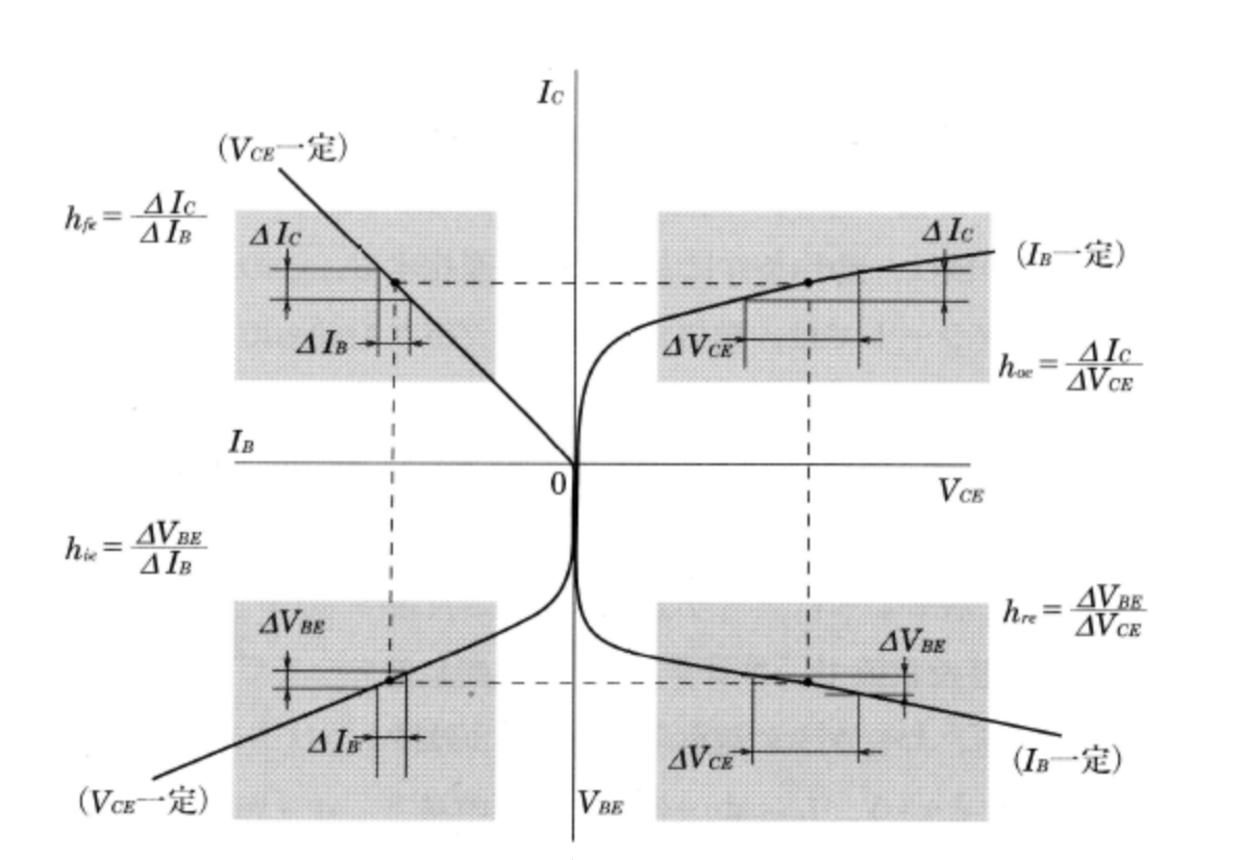
\includegraphics[width=0.5\textwidth]{figs/transistorCharacteristic.pdf}
  \caption{Transistor static characteristic diagram}
  \label{fig:my_label}
\end{figurehere}

\section{\textrm{Experimental procedures}}
使用装置:
可変直流定電流電源、可変直流定電圧電源、デジタル電圧計、可動コイル型直流電流 計、トランジスタ
\subsection{エミッター接地トランジスタの測定}
図2に、実験で用いたエミッター接地の測定回路を示す。測定回路内のトランジスターの入力と出力 にコンデンサーが並列に接続されているのは、トランジスターの利得による発振を防止するためである。
はじめに、ベース電流$I_B$を一定値に定めた状態で、コレクタ-エミッタ間電圧$V_{CE}$を変化させながらコレクタ電流$I_C$を測定した。次に、$V_{CE}$を一定値に定めた状態で、$I_B$を変化させながらベース-エミッタ間電圧$V_{BE}$を測定した。

\begin{figurehere}
  \centering
  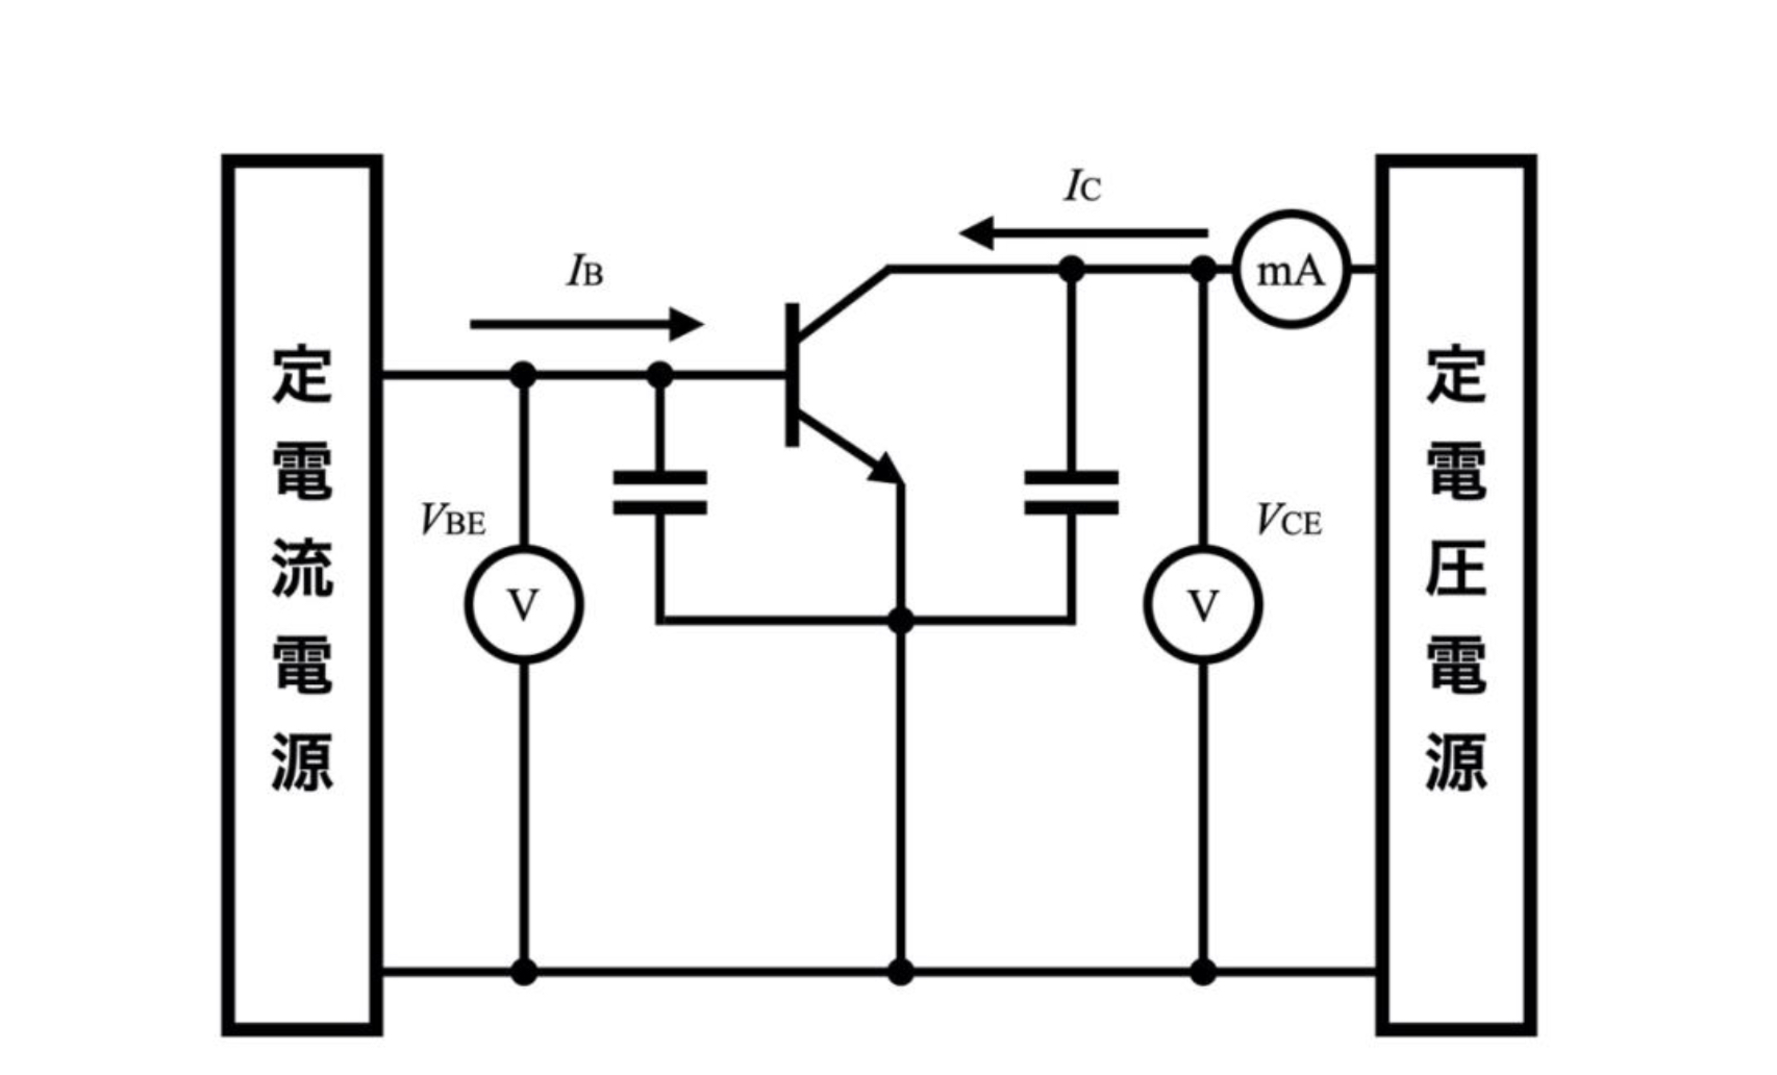
\includegraphics[width=0.5\textwidth]{figs/emitterCircuit.pdf}
  \caption{Emitter grounded circuit}
  \label{fig:my_label}
\end{figurehere}
\subsection{ベース接地トランジスタの測定}
図3に、実験で用いたベース接地回路を示す。コンデンサーがある理由は、2.1と同じである。はじめに、エミッタ電流$I_E$を一定値に定めた状態で、コレクタ-ベース間電圧$V_{CB}$を変化させながらコレクタ電流$I_C$を測定した。次に、$V_{CB}$を一定値に定めた状態で、$I_E$を変化させながらエミッタ-ベース間電圧$V_{EB}$を測定した。

\begin{figurehere}
  \centering
  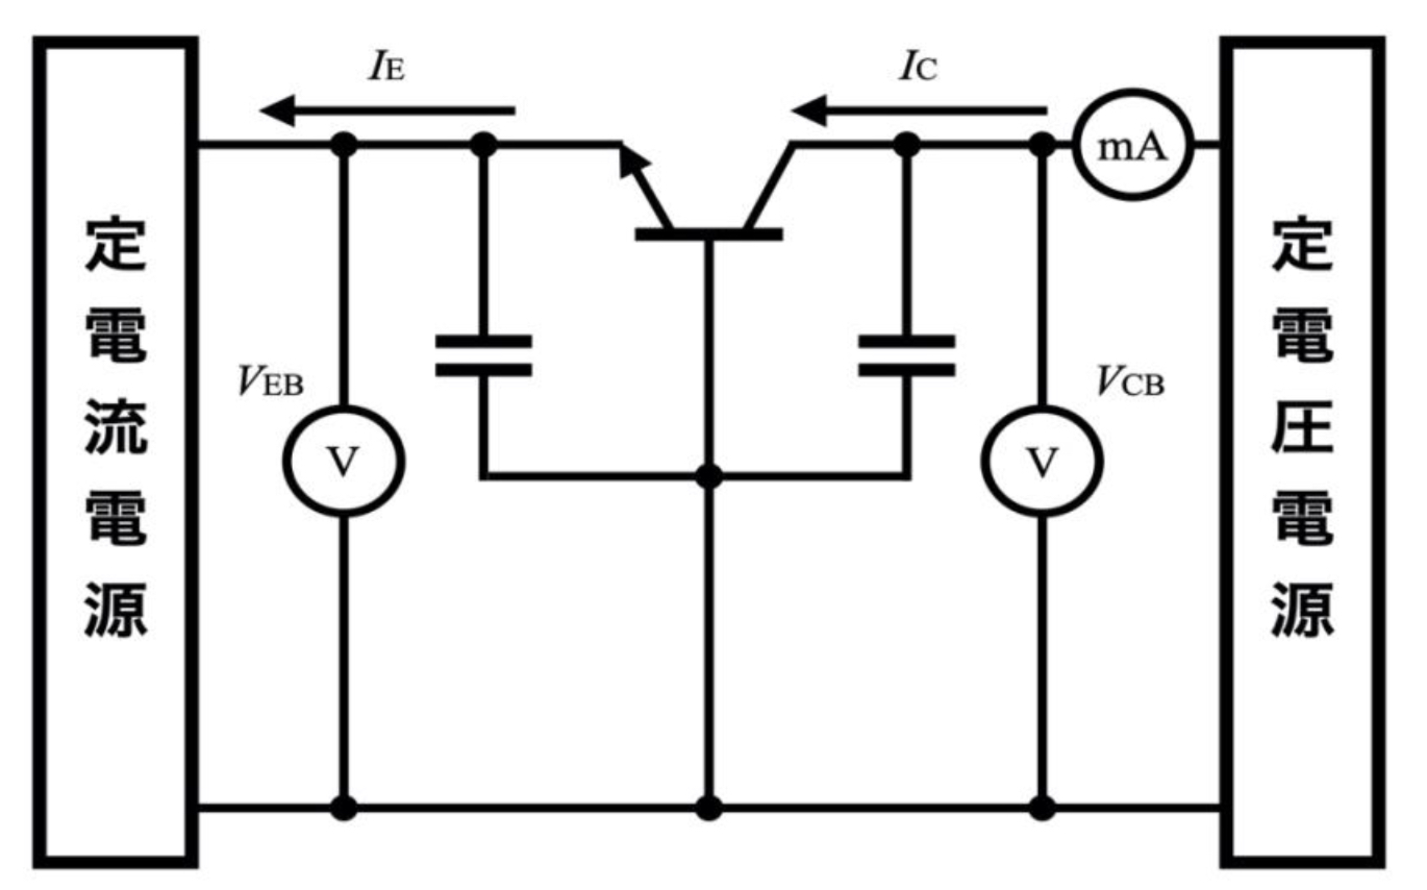
\includegraphics[width=0.4\textwidth]{figs/baseCircuit.pdf}
  \caption{Base grounded circuit}
  \label{fig:my_label}
\end{figurehere}


\end{multicols}
\section{\textrm{Results}}
\subsection{エミッター接地トランジスタ特性}
$I_B$を0, 20, 40, 60, 80, 100μAに定めた際の、$I_C$-$V_{CE}$特性の結果を図4に示す。
飽和領域と、活性領域が観測された。

\begin{figurehere}
  \centering
  \hspace*{0.5cm}
  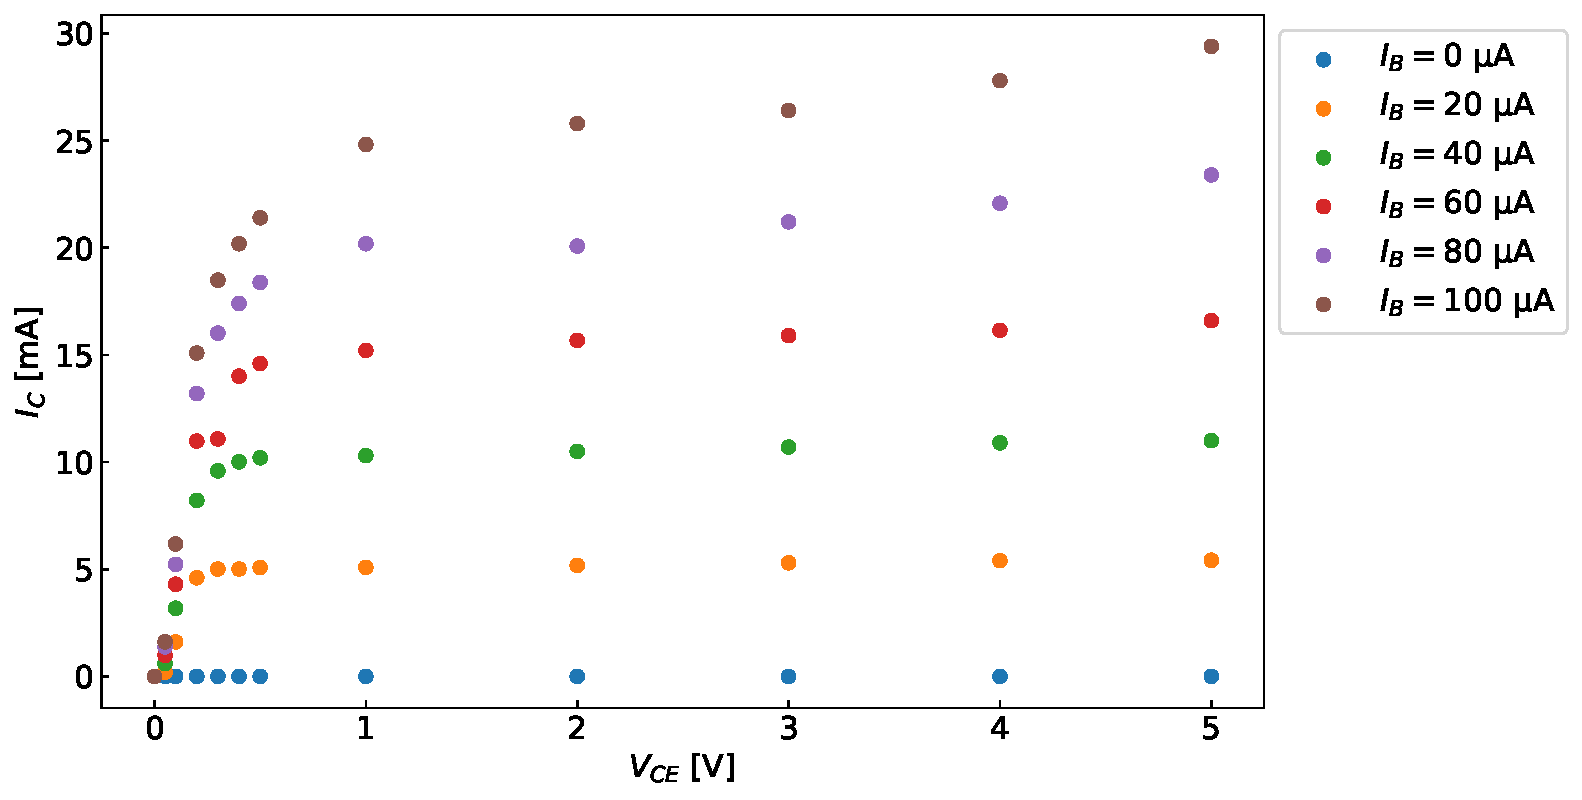
\includegraphics[width=0.9\textwidth]{figs/emitter1.pdf}
  \caption{$I_C$-$V_{CE}$ characteristics in emitter grounded circuit}
  \label{fig:my_label}
\end{figurehere}
$V_{CE}$を0, 0.1, 0.5, 1, 3Vに定めた際の、$I_B$-$V_{BE}$特性の結果を図5に示す。
ベース-ーエミッタ間電圧$V_{BE}$が増加するにつれて、ベース電流$I_B$が指数関数的に増加していることがわかる。一定の閾値電圧(約0.6〜0.7V)を超えると、ベース電流の増加が顕著になる。

\begin{figurehere}
  \centering
  \hspace*{0.5cm}
  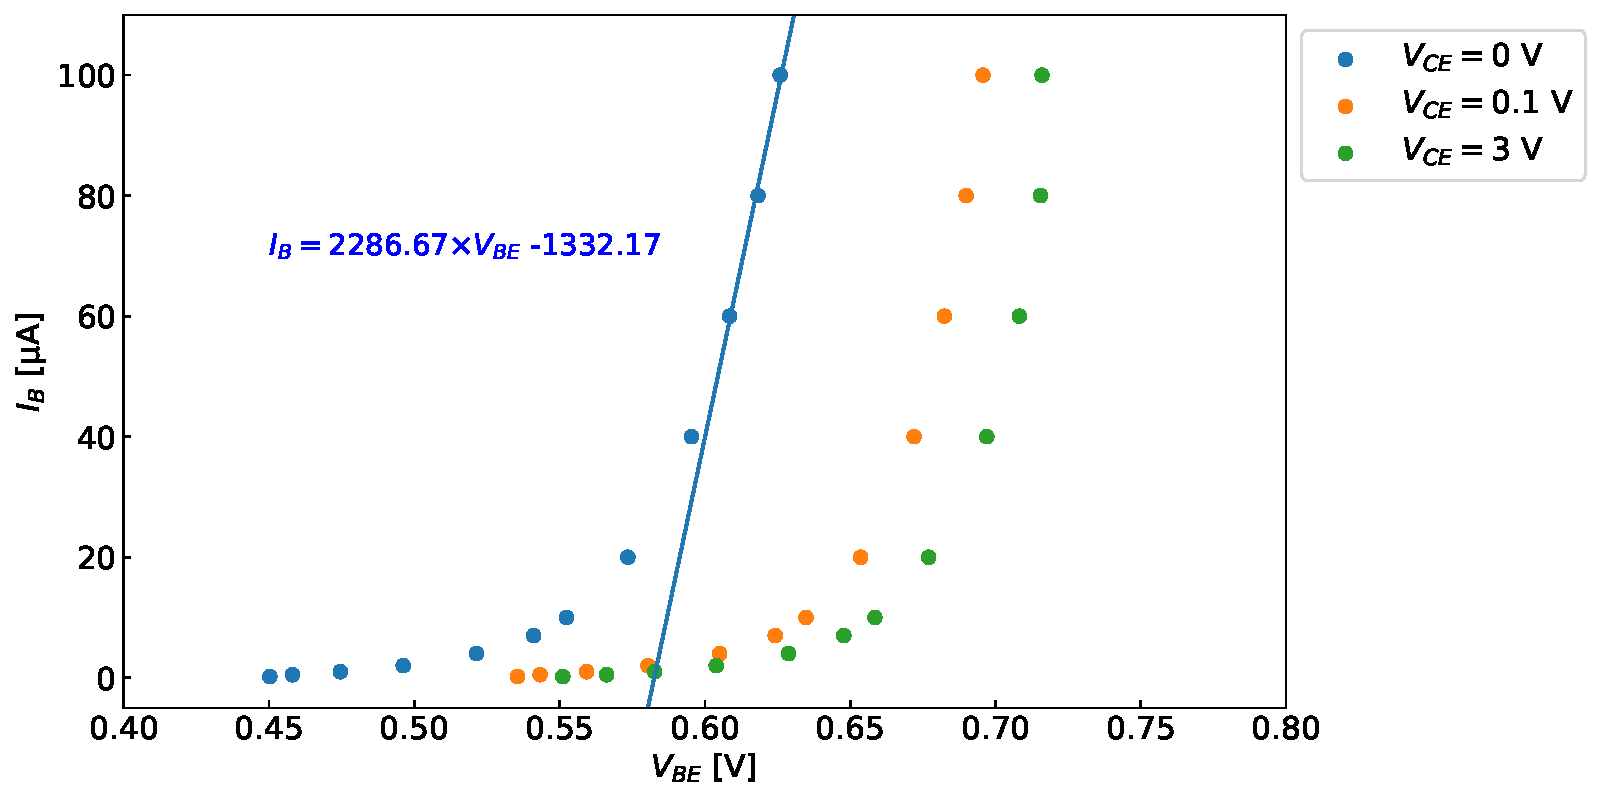
\includegraphics[width=0.9\textwidth]{figs/emitter2.pdf}
  \caption{$I_B$-$V_{BE}$ characteristics in emitter grounded circuit}
  \label{fig:my_label}
\end{figurehere}
\subsection{ベース接地トランジスタ特性}
$I_B$を0, 2, 4, 6, 8, 10μAに定めた際の、$I_C$-$V_{CE}$特性の結果を図6に示す。$V_{CE}$が一定まで上昇すると、$I_C$の値は飽和し、$I_B$の値を取っていることがわかる。

\begin{figurehere}
  \centering
  \hspace*{0.5cm}
  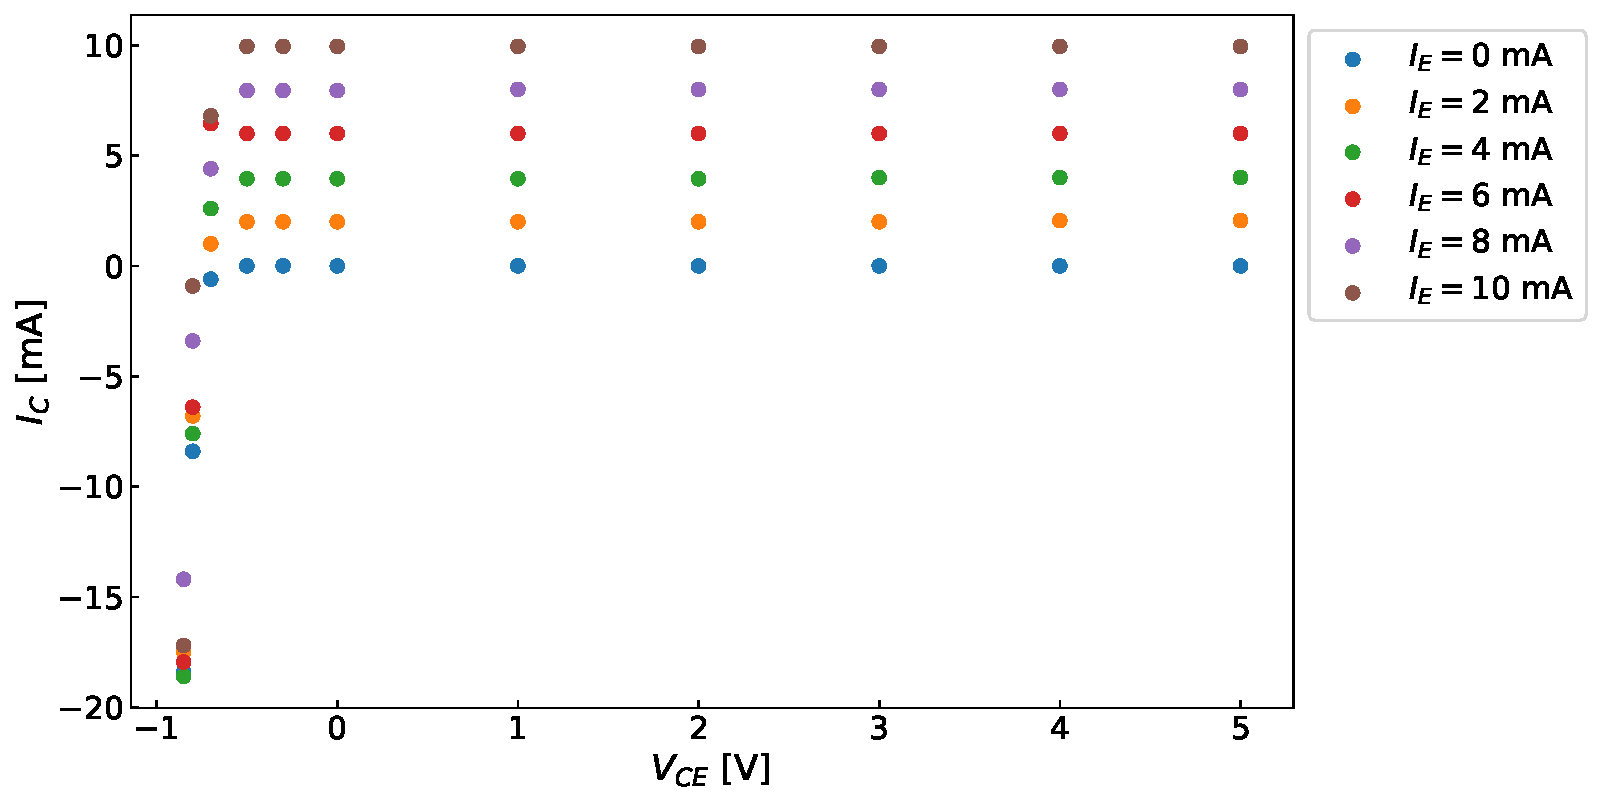
\includegraphics[width=0.9\textwidth]{figs/base1.pdf}
  \caption{$I_C$-$V_{CB}$ characteristics in a base-grounded circuit}
  \label{fig:my_label}
\end{figurehere}
\clearpage
$V_{CE}$を0, 0.1, 0.5, 1, 3Vに定めた際の、$I_B$-$V_{BE}$特性の結果を図5に示す。
ベース-ーエミッタ間電圧$V_{BE}$が増加するにつれて、ベース電流$I_B$が指数関数的に増加していることがわかる。

\begin{figurehere}
  \centering
  \hspace*{0.5cm}
  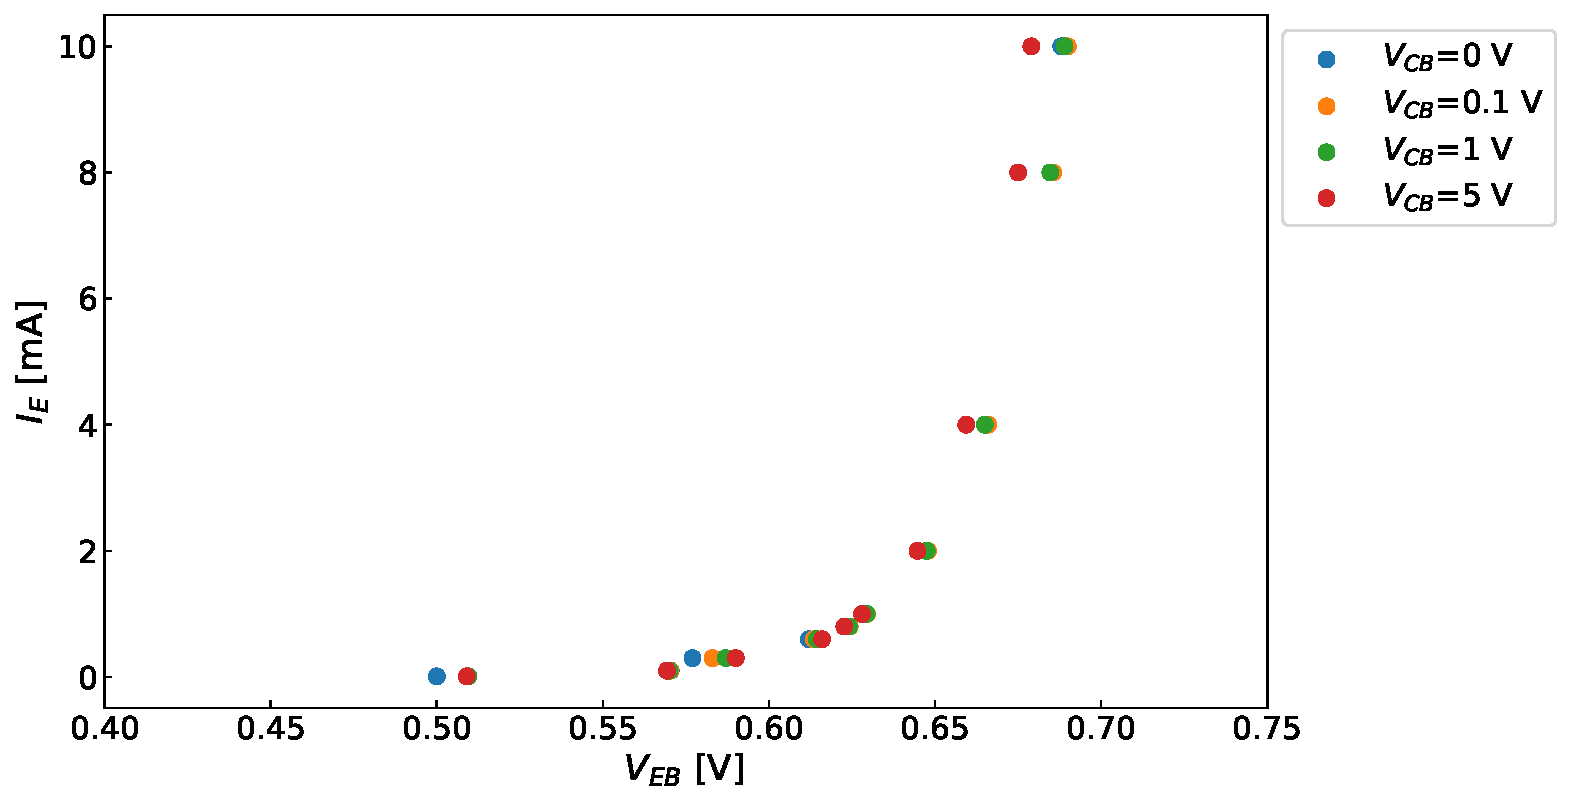
\includegraphics[width=0.9\textwidth]{figs/base2.pdf}
  \caption{$I_E$-$V_{EB}$ characteristics in a base-grounded circuit}
  \label{fig:my_label}
\end{figurehere}
\section{\textrm{Discussion}}
\subsection{hパラメータの計算}
エミッタ接地トランジスタにおいて、$I_C$-$V_{CE}$および、$I_B$-$V_{BE}$特性を、$I_C$-$I_B$および$V_{CE}$-$V_{BE}$特性に変換して、それぞれの特性の傾きからhパラメータを求めた。\\
直線的にプロットしている箇所を適当に選び、最小二乗法で近似直線をフィッティングした。図中の数式が近似直線の式である。\\

\begin{figurehere}
  \centering
  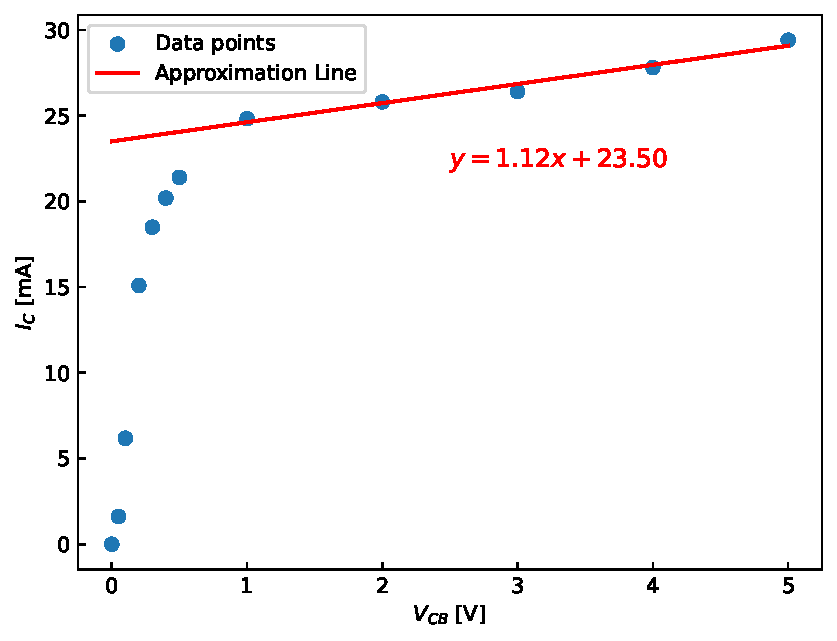
\includegraphics[width=0.565\textwidth]{figs/h_oe.pdf}
  \caption{$I_C$-$V_{CB}$ characteristics for $I_B$=100 μA in an emitter ground circuit}
  \label{fig:my_label}
\end{figurehere}
\begin{figurehere}
  \centering
  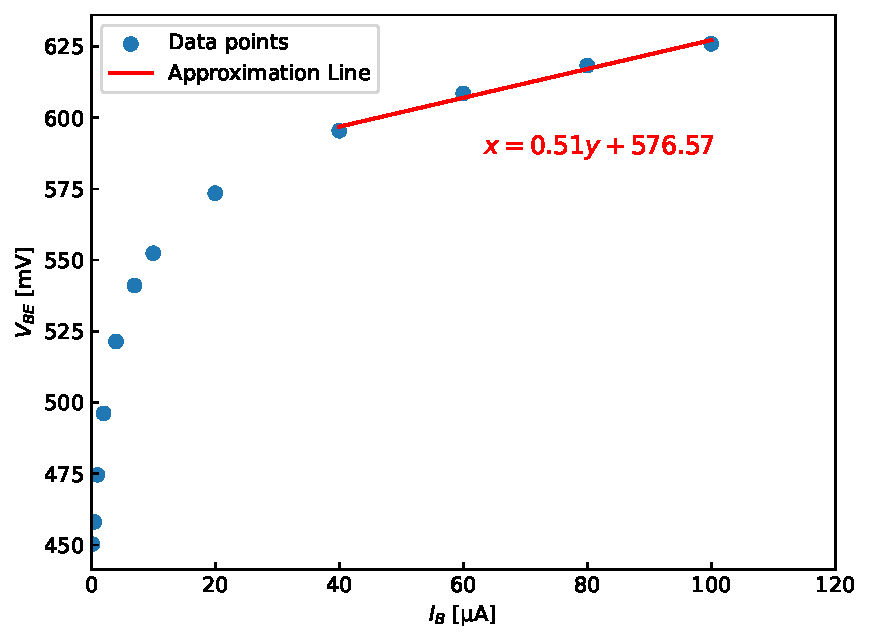
\includegraphics[width=0.585\textwidth]{figs/h_ie.pdf}
  \caption{$I_B$-$V_{BE}$ characteristics for $V_{CE}$=0 V in an emitter ground circuit}
  \label{fig:my_label}
\end{figurehere}

\begin{figurehere}
  \centering
  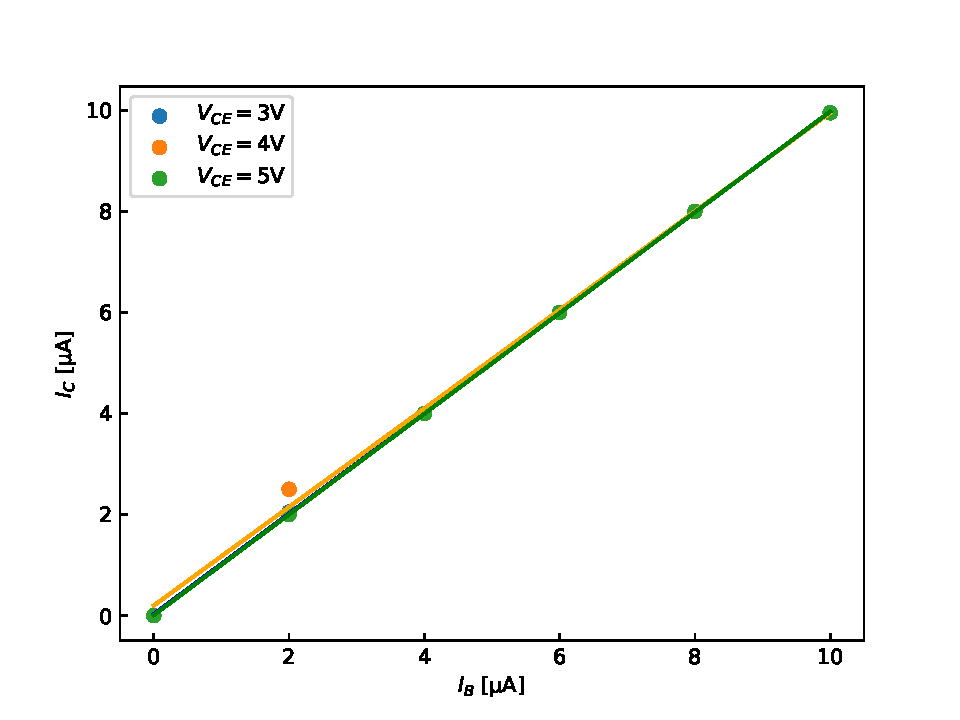
\includegraphics[width=0.65\textwidth]{figs/h_fe.pdf}
  \caption{$I_C$-$I_B$ characteristics for $V_{CE}$=4.0 V in an emitter ground circuit}
  \label{fig:my_label}
\end{figurehere}
\begin{figurehere}
  \centering
  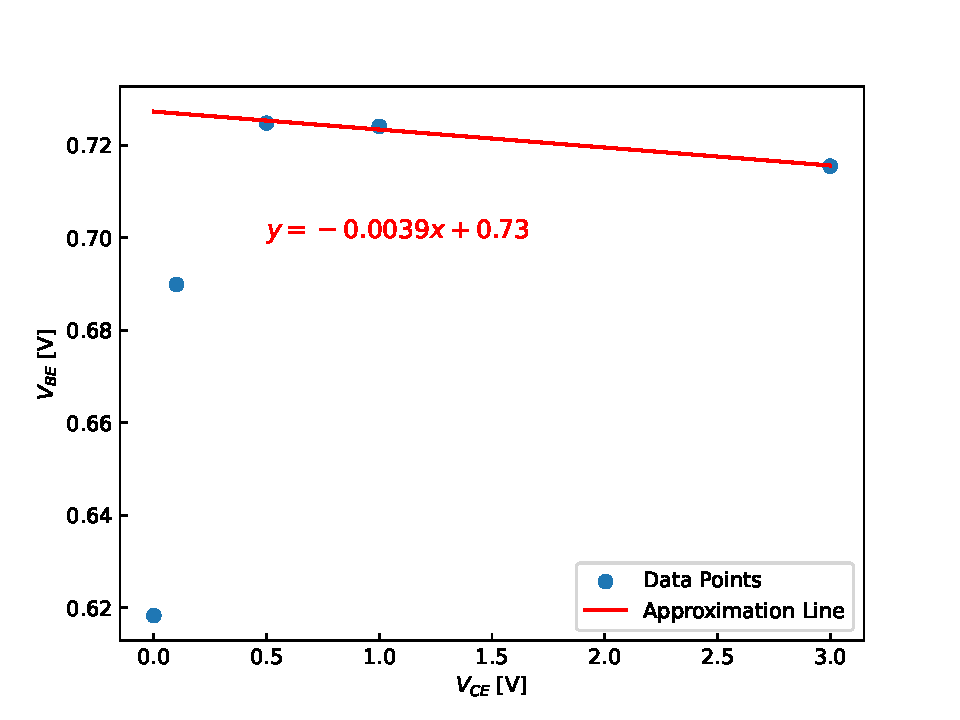
\includegraphics[width=0.65\textwidth]{figs/h_re.pdf}
  \caption{$V_{BE}$-$V_{CE}$ characteristic when $I_E$=80 μA in an emitter ground circuit}
  \label{fig:my_label}
\end{figurehere}
図11エミッタ接地トランジスタの$V_{BE}$-$V_{CE}$特性結果を見ると、理論上は正の傾きを持つ近似直線が引かれるはずであるが、実験結果からは負の傾きを持つ直線が引かれた。考えられる原因として、回路の問題、トランジスタの温度効果、トランジスタの劣化などが挙げられる。\\
結果、求められたhパラメータは以下のようになった。\\
$$
h_{oe}=1.1\times10^{-3} \text{S}
$$
$$
h_{fe}=270
$$
$$
h_{ie}=510\text{Ω}
$$
$$
h_{re}=-3.9\times10^{-3}
$$

\subsection{ベース接地トランジスタにおける$I_E$−$V_{EB}$特性の$V_{CB}$による相違}
$I_E$−$V_{EB}$特性において、$V_{CB}$=0のとき:
\begin{equation}
  I_E=I_S\left(\exp\left(-\frac{eV_{EB}}{kT}\right)-1\right)
\end{equation}
$I_S$は飽和電流、$e$は電気素量、$k$はボルツマン定数、$T$は絶対温度である。\\
$V_{CB}$が正のとき、コレクタ-ベース接合に逆バイアスがかかる。この逆バイアスによって、コレクタからベースへの少数キャリアの流れが制限され、結果的にエミッタ電流が減少する。
この効果による減少量は次式で表される:
\begin{equation}
  -\beta I_S\left(\exp\left(-\frac{eV_{CB}}{kT}\right)-1\right)
\end{equation}
この式では、トランジスタの増幅率$\beta$が重要な役割を果たしている。\\
$V_{CE}$=0と$V_{CE}>0$の相違は、$V_{CB}$の値によって、$I_E$の値が変化することによる。\\

\subsection{エミッタ接地トランジスタにおける$I_B$−$V_{BE}$特性の$V_{CB}$による相違}
\section{\textrm{Conclusion}}
エミッタ接地トランジスタとベース接地トランジスタの各特性を測定した。その結果として次のようなhパラメータが得られた:
$$
h_{oe}=1.1\times10^{-3} \text{S}, h_{fe}=270, h_{ie}=510\text{Ω}, h_{re}=-3.9\times10^{-3}
$$

さらに、ベース接地トランジスタでは、\( V_{CB} \)の値が\( I_E \)-\( V_{EB} \)特性に顕著な影響を及ぼし、エミッタ接地トランジスタでは、\( V_{CE} \)の値が\( I_B \)-\( V_{BE} \)特性に顕著な影響を及ぼすことがわかった。


\begin{thebibliography}{文献数}
  \bibitem{ID} http://www.gxk.jp/elec/musen/1ama/H32/html/H3212A06.html, 参照日2023/11/13
  \bibitem{ID2} 参考文献の名前・著者2
  \bibitem{ID3} 参考文献の名前・著者3
  \end{thebibliography}
\section{\textrm{Appendix}}
\begin{table}[H]
  \centering
  \caption{Measurement results of relationship between $I_C$ and $V_{CE}$ in emitter grounded circuits}
    \begin{tabular}{ccccccc}
    \multicolumn{1}{l}{$V_{CE}$ [V]} & \multicolumn{6}{c}{$I_C$ [mA]} \\
          & $I_B$=0 [µA] & 20    & 40    & 60    & 80    & 100 \\
    \midrule
    \midrule
    0.00  & 0.00  & 0.00  & 0.00  & 0.00  & 0.00  & 0.00 \\
    0.05  & 0.00  & 0.20  & 0.60  & 0.98  & 1.38  & 1.61 \\
    0.10  & 0.00  & 1.61  & 3.18  & 4.30  & 5.23  & 6.18 \\
    0.20  & 0.00  & 4.60  & 8.21  & 10.98 & 13.20 & 15.09 \\
    0.30  & 0.00  & 5.01  & 9.59  & 11.08 & 16.02 & 18.49 \\
    0.40  & 0.00  & 5.01  & 10.01 & 14.01 & 17.40 & 20.19 \\
    0.50  & 0.00  & 5.08  & 10.20 & 14.60 & 18.39 & 21.40 \\
    1.00  & 0.00  & 5.09  & 10.30 & 15.21 & 20.19 & 24.82 \\
    2.00  & 0.00  & 5.18  & 10.50 & 15.68 & 20.08 & 25.80 \\
    3.00  & 0.00  & 5.30  & 10.70 & 15.90 & 21.21 & 26.41 \\
    4.00  & 0.00  & 5.40  & 10.90 & 16.15 & 22.08 & 27.80 \\
    5.00  & 0.00  & 5.42  & 11.00 & 16.60 & 23.40 & 29.40 \\
    \end{tabular}%
  \label{tab:addlabel}%
\end{table}%
\begin{table}[H]
  \centering
  \caption{Measurement results of relationship between $I_B$ and $V_{BE}$ in emitter grounded circuits}
    \begin{tabular}{cccccc}
    $I_B$ [µA] & \multicolumn{5}{c}{$V_{BE}$ [mV]} \\
          & $V_{CE}$=0 [V] & 0.1   & 0.5   & 1.0   & 3.0 \\
    \midrule
    \midrule
    0.2   & 450.3 & 535.5 & 553.3 & 553.4 & 551.1 \\
    0.5   & 458.1 & 543.3 & 567.5 & 567.8 & 566.2 \\
    1.0   & 474.6 & 559.3 & 583.8 & 583.8 & 582.7 \\
    2.0   & 496.2 & 580.4 & 604.8 & 604.8 & 603.9 \\
    4.0   & 521.4 & 605.1 & 630.0 & 629.8 & 628.8 \\
    7.0   & 541.1 & 624.2 & 649.4 & 649.2 & 647.8 \\
    10    & 552.4 & 634.8 & 660.5 & 660.1 & 658.5 \\
    20    & 573.5 & 653.6 & 681.0 & 680.4 & 677.0 \\
    40    & 595.4 & 672.0 & 702.4 & 701.6 & 697.0 \\
    60    & 608.5 & 682.4 & 715.4 & 714.5 & 708.2 \\
    80    & 618.3 & 689.9 & 724.8 & 724.1 & 715.5 \\
    100   & 625.9 & 695.7 & 730.0 & 731.5 & 716.0 \\
    \end{tabular}%
  \label{tab:addlabel}%
\end{table}%
\begin{table}[H]
  \centering
  \caption{Measurement results of relationship between $V_{CB}$ and $I_C$ in a base-grounded circuit}
    \begin{tabular}{ccccccc}
    $V_{CB}$ [V] & \multicolumn{6}{c}{$I_C$ [mA]} \\
          & $I_E$=0 [mA] & 2     & 4     & 6     & 8     & 10 \\
    \midrule
    \midrule
    -0.85 & -18.40 & -17.50 & -18.60 & -17.95 & -14.20 & -17.20 \\
    -0.80 & -8.40 & -6.80 & -7.60 & -6.40 & -3.40 & -0.91 \\
    -0.70 & -0.60 & 1.00  & 2.60  & 3.40  & 4.40  & 6.80 \\
    -0.50 & 0.00  & 2.00  & 3.95  & 6.00  & 7.95  & 9.95 \\
    -0.30 & 0.00  & 2.00  & 3.95  & 6.00  & 7.95  & 9.95 \\
    0.00  & 0.00  & 2.00  & 3.95  & 6.00  & 7.95  & 9.95 \\
    1.00  & 0.00  & 2.00  & 3.95  & 6.00  & 8.00  & 9.95 \\
    2.00  & 0.00  & 2.00  & 3.95  & 6.00  & 8.00  & 9.95 \\
    3.00  & 0.00  & 2.00  & 4.00  & 6.00  & 8.00  & 9.95 \\
    4.00  & 0.00  & 2.05  & 4.00  & 6.00  & 8.00  & 9.95 \\
    5.00  & 0.00  & 2.05  & 4.00  & 6.00  & 8.00  & 9.95 \\
    \end{tabular}%
  \label{tab:addlabel}%
\end{table}%
\begin{table}[H]
  \centering
  \caption{Measurement results of relationship between $I_E$ and $V_{EB}$ in a base-grounded circuit}
    \begin{tabular}{ccccc}
    \multicolumn{1}{l}{$I_E$ [mA]} & \multicolumn{4}{c}{$V_{EB}$ [V]} \\
          & $V_{CB}$=0 [V] & 0.1   & 1     & 5.0 \\
    \midrule
    \midrule
    0.01  & 0.500 & 0.509 & 0.5095 & 0.5090 \\
    0.1   & 0.5704 & 0.5703 & 0.5700 & 0.5693 \\
    0.3   & 0.5770 & 0.5830 & 0.5870 & 0.5900 \\
    0.6   & 0.6120 & 0.6135 & 0.6144 & 0.6160 \\
    0.8   & 0.6240 & 0.6243 & 0.6241 & 0.6227 \\
    1.0   & 0.6290 & 0.6295 & 0.6294 & 0.6280 \\
    2.0   & 0.6477 & 0.6479 & 0.6475 & 0.6447 \\
    4     & 0.6650 & 0.6660 & 0.6650 & 0.6594 \\
    8     & 0.6850 & 0.6856 & 0.6847 & 0.6750 \\
    10    & 0.6880 & 0.6900 & 0.6890 & 0.6790 \\
    \end{tabular}%
  \label{tab:addlabel}%
\end{table}%
\end{document}